%-------------------------------------------------------------------------------

% This file is part of Code_Saturne, a general-purpose CFD tool.
%
% Copyright (C) 1998-2011 EDF S.A.
%
% This program is free software; you can redistribute it and/or modify it under
% the terms of the GNU General Public License as published by the Free Software
% Foundation; either version 2 of the License, or (at your option) any later
% version.
%
% This program is distributed in the hope that it will be useful, but WITHOUT
% ANY WARRANTY; without even the implied warranty of MERCHANTABILITY or FITNESS
% FOR A PARTICULAR PURPOSE.  See the GNU General Public License for more
% details.
%
% You should have received a copy of the GNU General Public License along with
% this program; if not, write to the Free Software Foundation, Inc., 51 Franklin
% Street, Fifth Floor, Boston, MA 02110-1301, USA.

%-------------------------------------------------------------------------------

\section{General description}
%----------------------------

        \subsection{Objective}
%-----------------------------

The aim of this case is to train the \CS  coupling with a thermal conduction and radiation
code SYRTHES on a simplified 2D problem. It corresponds to a natural convection inside a
sheath with different electric wires.

We can see with this test-case the conjugate heat transfer phenomenon between the solid
and fluid domains.

        \subsection{Remarks}
%---------------------------
$\bullet$ {\bf Remark - 1}:  create the \texttt{3disks2D} study directory, two subdirectories
\texttt{fluid} and \texttt{solid} as below:\\
\fbox{\begin{minipage}{\textwidth}\texttt{                                \\
\$ {\color{blue} code\_saturne create -s 3disks2D -c fluid --syrthes solid}
}\end{minipage} }

$\bullet$ {\bf Remark - 2}:  The fluid mesh must be copied in the directory \texttt{MESH}.
The solid mesh must be copied in the subdirectory \texttt{solid}.

$\bullet$ {\bf Remark - 3}: launch the \syrthes Graphical User Interface (Gui)
(\texttt{\$ {\color{blue}syrthes.gui \&}}) inside the subdirectory \texttt{solid} for the first
solid computation alone.

$\bullet$ {\bf Remark - 4}: launch the \CS Graphic User Interface (GUI) inside the
subdirectory \texttt{fluid} for the fluid computation alone.

$\bullet$ {\bf Remark - 5}: launch the \CS-\syrthes coupling computation with the
\texttt{{\color{blue}runcase\_coupling}} script.

        \subsection{Description of the configuration}
%-----------------------------------------------

The 2D configuration represents a simplification of the real 3D geometry of the wires inside an electric sheath.
As we can see, we have 3 different wires represented as 3 different disks inside a bigger disk for the sheath.
We assume that the 3 disks are in contact with an air flow inside the electric sheath.

The geometry is shown on figure \ref{config}.


\begin{figure}[h!]
\begin{center}
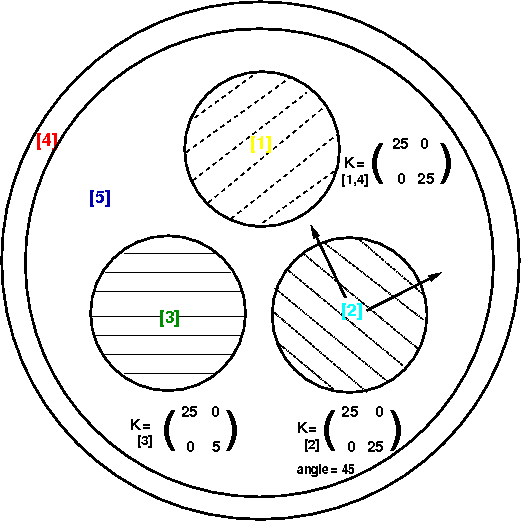
\includegraphics[width=6cm,height=6.0cm]{case6_geometry-3rond2d}
\caption{Geometry of the test-case with [1,2,3,4] the solid domain and [5] the fluid domain.
The 4 disk physical properties are specified for the solid domain.}
\label{config}
\end{center}
\end{figure}

For the fluid domain, there are two symmetry conditions and walls conditions imposed to the faces coupling with
the solid domain. We have no velocity imposed to create movement inside the fluid area
and gravity force is taken into account.

Nevertheless, we define a density which is variable in function of the temperature for the air flow.
The 3 disks, which are warmer than the air flow, generate a temperature difference creating a fluid movement.
The warmer air flow is moving to the top and the colder air flow to the bottom of the fluid domain.

With this test-case, we can easily observe the effect of the solid disks on the air flow contained in the electric sheath.

%\newpage

        \subsection{Characteristics}
%----------------------------------

$\bullet${~~\bf \underline{Solid domain}:}\\

The initial and boundary conditions to choose without conjugate heat transfer for the solid domain are defined hereafter:

\begin{center}
\begin{tabular}{|l|ccc|}
\hline
         Initial conditions                  &                    &\quad &                               \\
\hline
\hline
         Temperature condition               &   $T_{ini,s} = 20$\degresC &      &                            \\
\hline
\end{tabular}\\
\end{center}

\begin{center}
\begin{tabular}{|l|lcc||c|}
\hline

         Boundary conditions                 &  value             &\quad &                           & surface reference    \\
\hline
\hline
       Heat exchange conditions ($q_{w,ext}$)& $T_{ext} = 90$\degresC. &;\quad & $h_{ext}= 1000 (W/m^2.K)$ & color 2 or 5 or 8    \\
\hline
\end{tabular}\\
\end{center}

Characteristics of the solid domain with the 4  different disks (1 to 3 for the electric wires and 4 for the disk for the electric sheath): \\
\begin{center}
\begin{tabular}{|l|l|ccc||c|}
\hline
       &  Conductivity  type      &   values      &   (W/m/\degresC)        &                   & volume reference  \\
\hline
\hline
disk 1 & isotropic                & $k_{11}= 25$ &                  &                   & color 1\\
\hline
disk 2 & orthotropic              & $k_{11}= 25$ &; $k_{22}=5$       &                   & color 2\\
\hline
disk 3 & orthotropic              & $k_{11}= 25$ &; $k_{22}=5$       & $\alpha = 45^o$& color 3 \\
\hline
disk 4 & anisotropic              & $k_{11}= 25$ &                  &                   & color 4\\
\hline
\end{tabular}\\
\end{center}

\begin{center}
\begin{tabular}{|l|cc|}
\hline
  Physical properties      &   values   &                           \\
\hline
\hline
 Density [$\rho$]                  &     $7700$  &$(kg/m^2)$        \\
\hline
 Specific heat [$C_p$]             &     $460$   &$(J/kg/m^3)$      \\
\hline
\end{tabular}\\
\end{center}

$\bullet${~~\bf \underline{Fluid domain}:}\\

The characteristics of the air flow inside the fluid domain are defined as following:

\begin{center}
\begin{tabular}{|l|l|}
\hline
  Thermophysical models       &   choosen type                         \\
\hline
\hline
  Time step                   &  constant in time and uniform in space \\
\hline
 Turbulence model             &  $\varepsilon$ -k                      \\
\hline
  Scalar                      & Temperature (\degresC)                 \\
\hline
\end{tabular}\\
\end{center}

The initial and boundary conditions to choose without conjugate heat transfer for the solid domain are defined below:

\begin{center}
\begin{tabular}{|l|c|}
\hline
         Initial conditions                  &                       \\
\hline
\hline
         Temperature condition               &   $T_{ini,f} = 20$\degresC. \\
\hline
\end{tabular}\\
\end{center}

\begin{center}
\begin{tabular}{|l|lcc||c|}
\hline

         Boundary conditions                 &    values                &  &                              & surface reference \\
\hline
\hline
       Walls (Heat exchange $q_{w,ext}$)    & $T_{ext} = 30$\degresC         &; & $h_{ext}= 10 (W/m^2.K)$      & color 1           \\
\hline
       Symmetry                              &                          &  &                              & color 2 or 3      \\
\hline
\end{tabular}\\
\end{center}

In this case, the fluid density is function of the temperature, the following ideal gas law is specified in the Graphical User Interface (GUI):
\begin{equation}
\rho = \frac{p_0}{R_g~(T+ 273.15)}
\end{equation}
where $\rho$ is the density, $T$ is the temperature (\degresC), ideal gas constant $R_g = 287~(m^2.s^{-2}.K^{-1})$,
$p_0=101325~(Pa)$ the reference pressure choosen as $p\approxeq p_{atmos}$.


        \subsection{Mesh characteristics}
%---------------------------------------

$\bullet${~~\bf \underline{Description of the solid mesh}:}\\

The solid mesh used in the conduction problem contains 11688 nodes ($P_1$ discretization) and 5688 elements.
We have to take care of the references allowing to identify materials properties and boundary conditions which
 are specified in this solid mesh by reference colors.

{\bfseries Type}: unstructured mesh
\vspace{0.1in}
{\bfseries Mesh generator used}: SIMAIL
{\bfseries Color definition}: see figure \ref{fige1_e5}.

\begin{figure}[h!]
\begin{center}
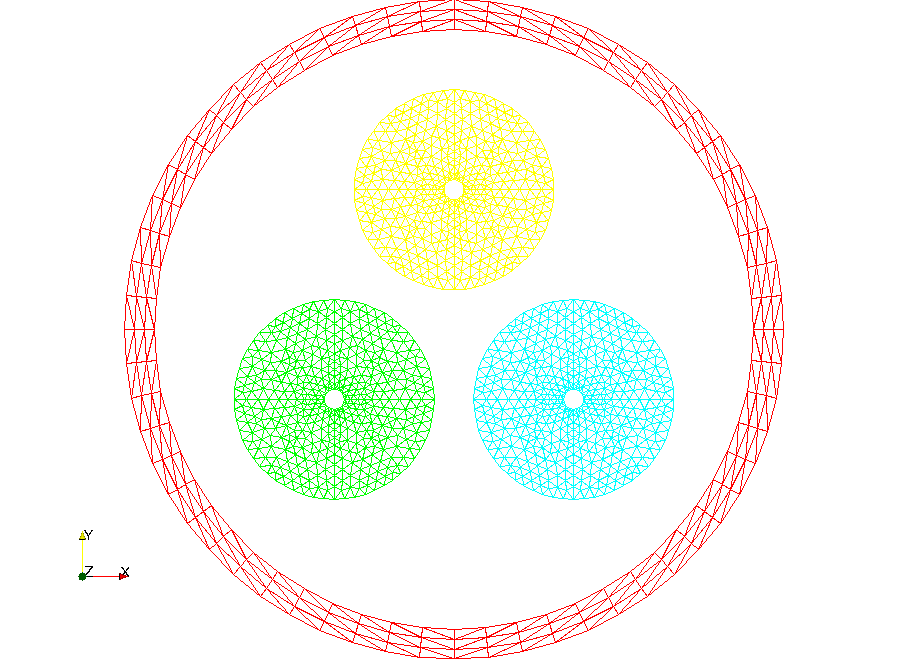
\includegraphics[width=8cm]{case6_solid-mesh-color}
\caption{Colors of the boundary faces}
\label{fige1_e5}
\end{center}
\end{figure}

$\bullet${~~\bf \underline{Description of the fluid mesh}:}\\

The fluid mesh contains 3866 nodes. We have to apply the
{\bf check mesh} available in the \CS Graphical User Interface to
check the quality criteria and identify the reference colors
associated to the boundary conditions.

{\bfseries Type}: unstructured mesh
{\bfseries Mesh generator used}: SIMAIL
{\bfseries Color definition}: see figure \ref{fige1_e5}.

\begin{figure}[h!]
\begin{center}
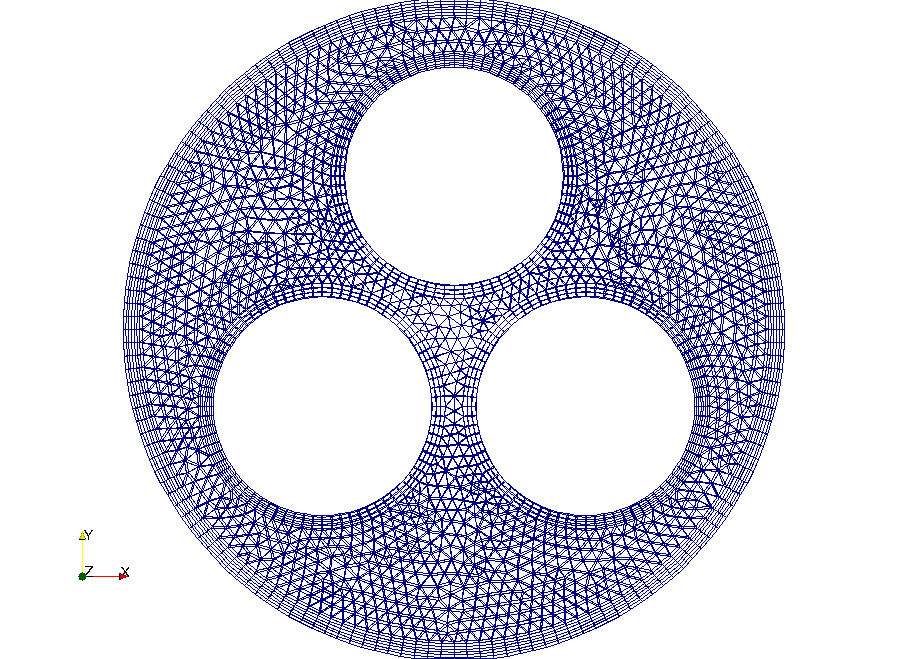
\includegraphics[width=8cm]{case6_color-fluid-mesh}
\caption{Colors of the boundary faces}
\label{fige1_e5}
\end{center}
\end{figure}

\newpage
%-----------------------------
\section{CASE 6: 3 2D disks}
%-----------------------------

The post-processing containing the ``temperature'' field will be post-processed on a
sub-mesh with ParaView. A 2D clip plane will also be extracted along the symmetry plane of the fluid
domain and temperature will be written on it.


        \subsection{Parameters}
%------------------------------
All the parameters necessary to this study can be defined through the \CS (GUI)
and \syrthes (Gui) respectively, as below:

\begin{center}
\begin{tabular}{|l|c|}
\hline
\multicolumn{2}{|c|}{ Numerical parameters of {\bf solid computation}} \\
\hline
Reference time step  & $0.1$ (s) \\
\hline
Number of iterations & 100 \\
\hline
\hline
\multicolumn{2}{|c|}{ Numerical parameters of {\bf fluid computation}} \\
\hline
Reference time step  & $0.1$ (s) \\
\hline
Number of iterations & 100 \\
\hline
\end{tabular}\\
\end{center}

These numerical time steps and iterations number have been defined to run the
fluid and solid computations independently one from each other.
Thus, we can test the setting data for the fluid computation with \CS and
 the solid conduction computation with SYRTHES.
After that we will be able to run the coupling computation with the computation
option {\bf conjugate heat transfer} activated on both data setting.

        \subsection{Output management}
%-------------------------------------
The standard options for output management will be used. Only one monitoring point
will be created for the solid conduction computation at the following coordinates:

\begin{center}
\begin{tabular}{|c|c|c|}
\hline
Probe & $x$ (m) & $y$(m)    \\
\hline
1      & 0.003  & -1.2       \\
\hline
\end{tabular}
\end{center}

For this probing we choose to save the temperature value every 10 time steps and
the temperature field every 25 time steps.


        \subsection{Coupling computation}
%----------------------------------------

The  numerical parameters used for the coupling computation must be modified to be sure
 to see the conjugate heat transfer phenomenon between the solid and fluid domains.
For this reason, we increase the iterations number and the time step for the fluid
and solid data setting.

By default, the smaller iterations number will be used to drive the coupling computation.
If we choose an iterations number of 10000 for the fluid domain and 5000 for the solid
domain, the coupling computation will be stopped after 5000 instead of 10000.

\begin{center}
\begin{tabular}{|l|c|}
\hline
\multicolumn{2}{|c|}{ Numerical parameters of {\bf solid computation}} \\
\hline
Reference time step  & $0.5$ (s) \\
\hline
Number of iterations & 50000 \\
\hline
\hline
\multicolumn{2}{|c|}{ Numerical parameters of {\bf fluid computation}} \\
\hline
Reference time step  & $0.5$ (s) \\
\hline
Number of iterations & 50000 \\
\hline
\end{tabular}\\
\end{center}

        \subsection{Results}
%---------------------------

Figure \ref{fige2_e5} shows the evolution of the temperature in the solid domain
without {\bf conjugate heat transfer} with the fluid domain. We have represented
below the evolution of the temperature in the fluid domain without coupling with
SYRTHES.

\begin{figure}[h!]
\begin{center}
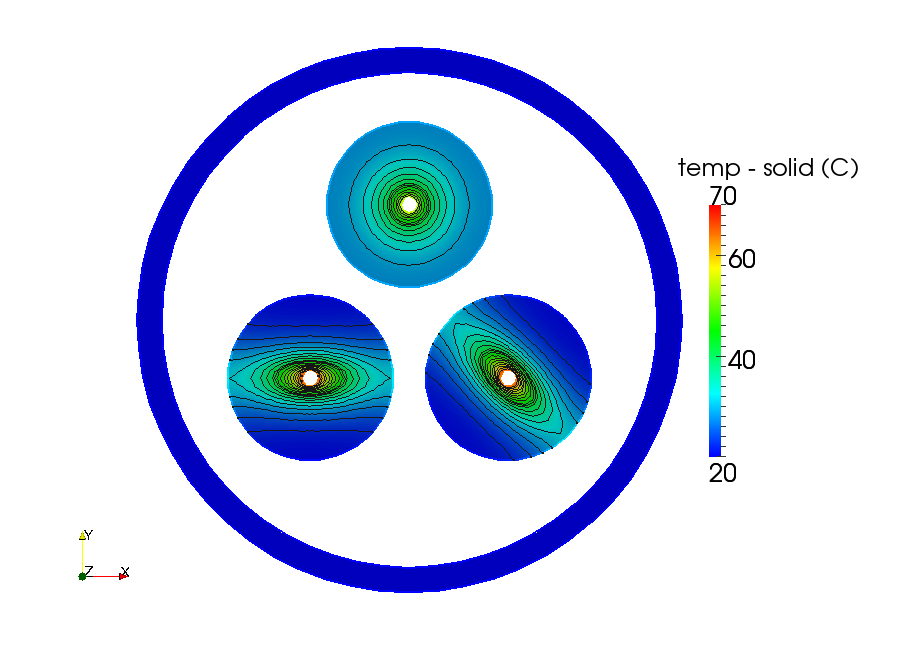
\includegraphics[width=10cm]{case6_Visu2d-solid-temp}
\caption{The temperature evolution in the {\bf solid domain without coupling method} }
\label{fige4_e5}
\end{center}
\end{figure}

\begin{figure}[h!]
\begin{center}
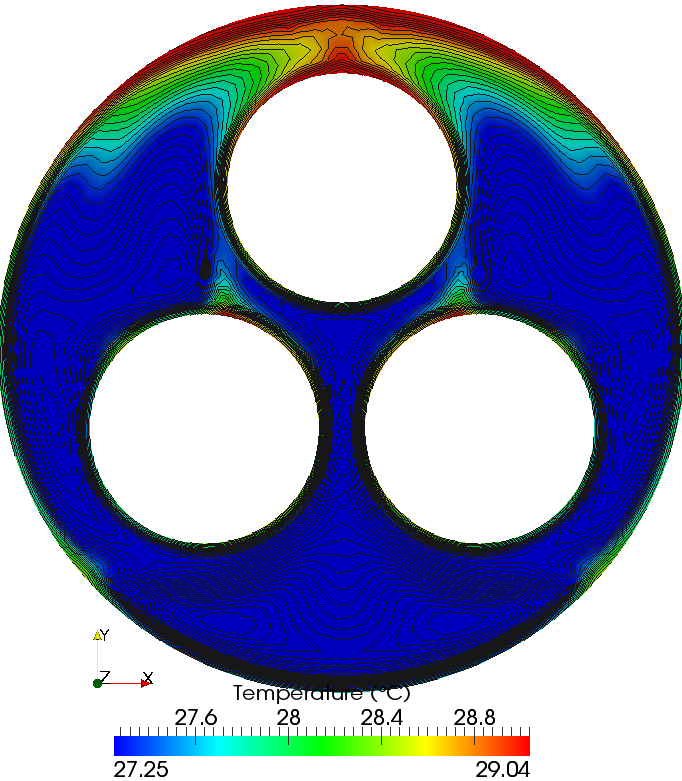
\includegraphics[width=6cm]{case6_Visu2d_Temp_fluid}
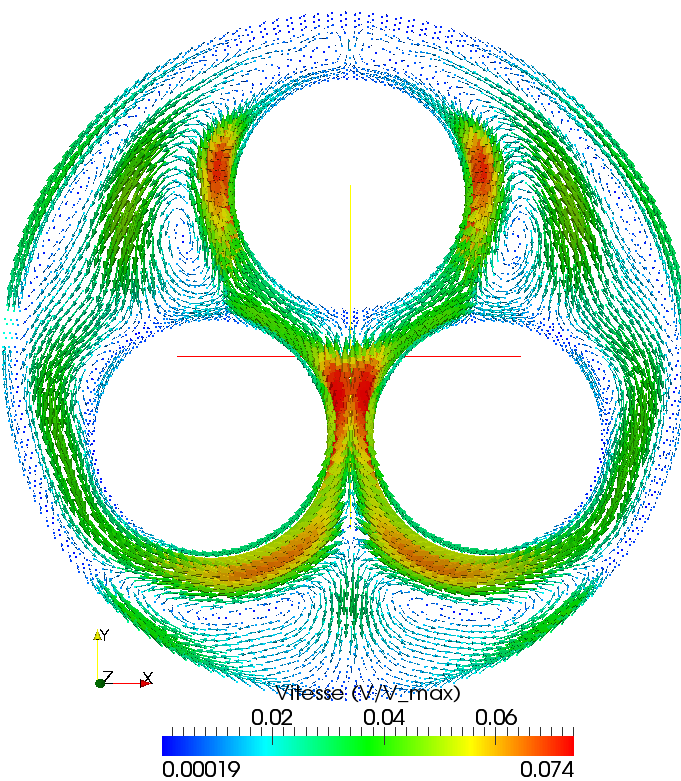
\includegraphics[width=6cm]{case6_Visu2d_Vec_fluid}
\caption{The temperature evolution in the {\bf fluid domain without coupling method}}
\label{fige4_e5}
\end{center}
\end{figure}

%\newpage

Figure \ref{fige2_e5} shows the evolution of the temperature in the solid and fluid area with
the {\bf conjugate heat transfer activated}. The natural convection in the fluid domain due to the
temperature difference imposed by the solid disks is clearly visible with the velocity field and vector.

\begin{figure}
\begin{center}
\begin{tabular}{c}
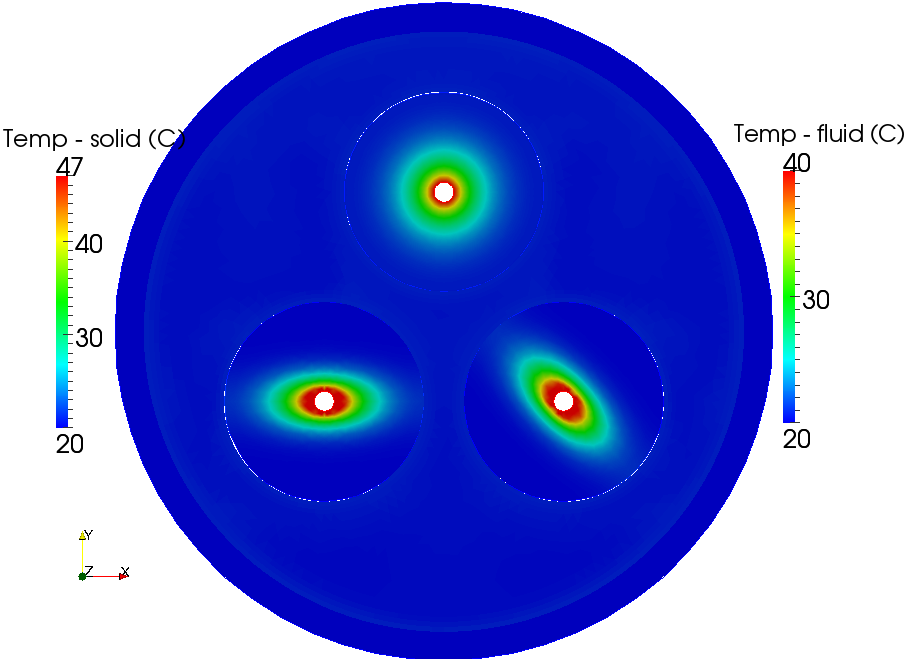
\includegraphics[width=9cm]{case6_Visu2D-coupling-temp00} \\
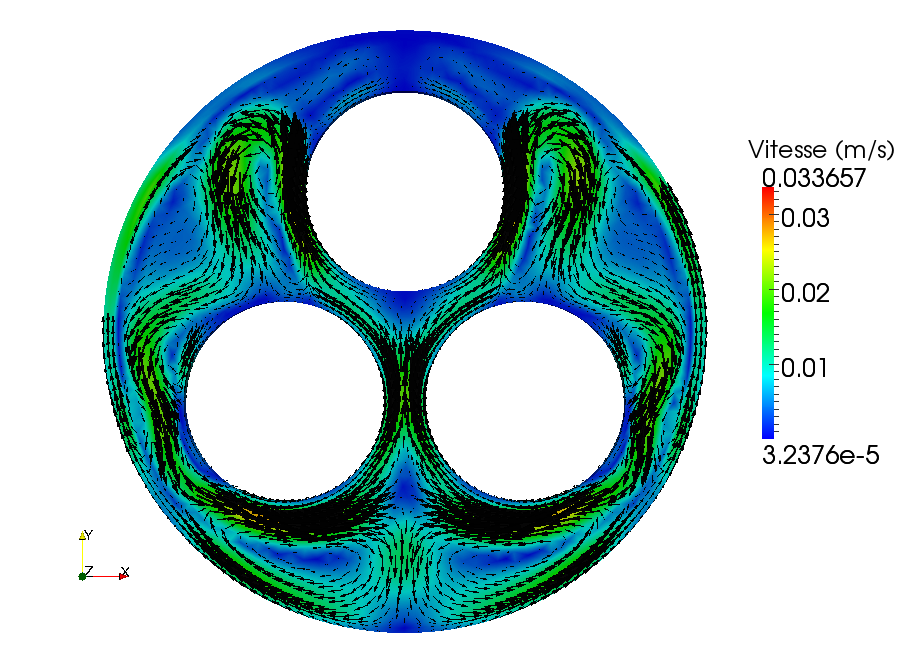
\includegraphics[width=9cm]{case6_Visu2D-coupling-Vec00}  \\
\end{tabular}
\caption{Evolution of temperature}
\label{fige2_e5}
\end{center}
\end{figure}




